\documentclass[12pt,a4paper]{article}

\usepackage[indonesian]{babel}
\usepackage[utf8]{inputenc}
\usepackage[T1]{fontenc}
\usepackage{lmodern}
\usepackage[a4paper,margin=2.5cm]{geometry}
\usepackage{graphicx}
\usepackage{float}
\usepackage{caption}
\usepackage{xcolor}
\usepackage{booktabs}
\usepackage{enumitem}
\usepackage[hidelinks]{hyperref}
\usepackage{fancyhdr}

\graphicspath{{screenshots/}}
\setlength{\parindent}{0pt}
\setlength{\parskip}{6pt}
\captionsetup{font=small,labelfont=bf}

\pagestyle{fancy}
\fancyhf{}
\lhead{Laporan P10}
\rhead{Observability Laravel dan Docker Compose}
\cfoot{\thepage}

\newcommand{\screenshot}[3]{
  \begin{figure}[H]
    \centering
    \includegraphics[width=\textwidth,height=0.30\textheight,keepaspectratio]{#1}
    \caption{#2}
    \label{fig:#3}
  \end{figure}
}

\title{
  \textbf{Laporan P10}\\
  \large Observability Laravel dan Docker Compose
}
\author{
  Nawwaf Zayyan Musyafa\\
  NIM: 24/540567/SV/24877
}
\date{6 November 2026}

\begin{document}

\maketitle
\thispagestyle{empty}

\begin{center}
\textbf{Repository:}\\
\url{https://github.com/davudumon/uts-pl-24-540567-SV-24877}
\end{center}

\tableofcontents
\newpage

\section{Tujuan}

Pekerjaan ini menerapkan observability pada aplikasi perpustakaan berbasis Laravel
yang dijalankan menggunakan Docker Compose. Ruang lingkupnya meliputi:

\begin{enumerate}[label=\arabic*.]
  \item mengarahkan log Laravel ke standard output container;
  \item menambahkan log terstruktur dengan konteks pelaku, aksi, dan alasan;
  \item menyediakan endpoint \texttt{/health} yang benar-benar memeriksa database dan cache;
  \item memasang healthcheck pada service Docker Compose;
  \item membuktikan kondisi sehat, gagal ketika database dimatikan, dan pulih kembali;
  \item membatasi ukuran log menggunakan \texttt{max-size} dan \texttt{max-file}.
\end{enumerate}

\section{Implementasi}

\subsection{Logging ke standard output}

Channel logging Laravel menggunakan Monolog dengan \texttt{JsonFormatter} dan stream
\texttt{php://stdout}. Dengan demikian, log dapat dibaca menggunakan:

\begin{verbatim}
docker compose logs backend
\end{verbatim}

Konfigurasi Docker Compose menggunakan driver \texttt{json-file} dengan pembatasan:

\begin{itemize}
  \item \texttt{max-size: 10m}, yaitu ukuran maksimum satu file log;
  \item \texttt{max-file: 3}, yaitu jumlah file log yang dipertahankan.
\end{itemize}

\subsection{Log terstruktur}

Log ditambahkan pada alur penting operasi buku:

\begin{itemize}
  \item \textbf{INFO} ketika buku berhasil disimpan;
  \item \textbf{WARNING} ketika validasi input buku gagal;
  \item \textbf{ERROR} ketika pemeriksaan atau akses database gagal.
\end{itemize}

Konteks log menggunakan field \texttt{who}, \texttt{action}, dan \texttt{reason}.
Nilai password, token, cookie, dan data pribadi tidak dicatat.

\subsection{Endpoint kesehatan}

Endpoint \texttt{GET /health} menjalankan dua pemeriksaan:

\begin{enumerate}
  \item query \texttt{select 1} melalui koneksi database;
  \item operasi \texttt{put/get} pada cache.
\end{enumerate}

Jika kedua pemeriksaan berhasil, endpoint mengembalikan HTTP 200 dan status
\texttt{healthy}. Jika salah satu gagal, endpoint mengembalikan HTTP 503 dan
menyebutkan komponen yang gagal.

\section{Bukti Kondisi Sehat}

\screenshot{Screenshot 2026-11-06 193423.png}
{Semua service Docker Compose berstatus healthy}
{healthy-services}

Gambar~\ref{fig:healthy-services} menunjukkan bahwa service \texttt{backend},
\texttt{db}, dan \texttt{frontend} berjalan dengan status \texttt{healthy}.
Ini membuktikan bahwa healthcheck Compose berhasil dijalankan pada kondisi normal.

\screenshot{Screenshot 2026-11-06 193521.png}
{Respons endpoint health pada kondisi sehat}
{health-healthy}

Respons pada Gambar~\ref{fig:health-healthy} menunjukkan:

\begin{verbatim}
{
  "status": "healthy",
  "checks": {
    "database": "ok",
    "cache": "ok"
  }
}
\end{verbatim}

Database dan cache sama-sama berhasil diperiksa sehingga endpoint mengembalikan
status sehat.

\section{Bukti Log Terstruktur}

\screenshot{Screenshot 2026-11-06 193759.png}
{Log backend dalam format JSON melalui docker compose logs}
{structured-log}

Gambar~\ref{fig:structured-log} memperlihatkan log JSON
\texttt{Book saved}. Log tersebut memiliki konteks:

\begin{itemize}
  \item \texttt{who: authenticated\_user}: pelaku adalah pengguna yang sudah
  terautentikasi;
  \item \texttt{action: create\_book}: aksi yang sedang dilakukan adalah membuat
  buku;
  \item \texttt{reason: book\_created\_successfully}: alasan log dibuat adalah
  penyimpanan berhasil.
\end{itemize}

Format JSON dan kemunculan log pada \texttt{docker compose logs} membuktikan bahwa
log dikeluarkan ke standard output container, bukan hanya ke file internal.

\section{Bukti Konfigurasi Healthcheck dan Rotasi Log}

\screenshot{Screenshot 2026-11-06 193849.png}
{Konfigurasi pembatasan ukuran log}
{log-rotation}

Gambar~\ref{fig:log-rotation} memperlihatkan konfigurasi:

\begin{verbatim}
logging:
  driver: json-file
  options:
    max-file: "3"
    max-size: 10m
\end{verbatim}

\screenshot{Screenshot 2026-11-06 193914.png}
{Parameter healthcheck database}
{db-healthcheck}

Gambar~\ref{fig:db-healthcheck} menunjukkan parameter healthcheck database:
\texttt{timeout: 5s}, \texttt{interval: 5s}, \texttt{retries: 20}, dan
\texttt{start\_period: 30s}. Pemeriksaan menggunakan \texttt{mysqladmin ping},
sehingga status database tidak hanya bergantung pada proses container yang hidup.

\section{Bukti Kondisi Sakit}

\screenshot{Screenshot 2026-11-06 194408.png}
{Status service setelah database dimatikan}
{database-stopped}

Database dimatikan secara sengaja menggunakan:

\begin{verbatim}
docker compose stop db
\end{verbatim}

Pada Gambar~\ref{fig:database-stopped}, container database berhenti dan backend
berubah menjadi \texttt{unhealthy}. Frontend tetap \texttt{healthy} karena
healthcheck frontend memeriksa kemampuan Nginx menyajikan halaman, sedangkan
healthcheck backend memeriksa endpoint yang bergantung pada database dan cache.

\begin{figure}[H]
  \centering
  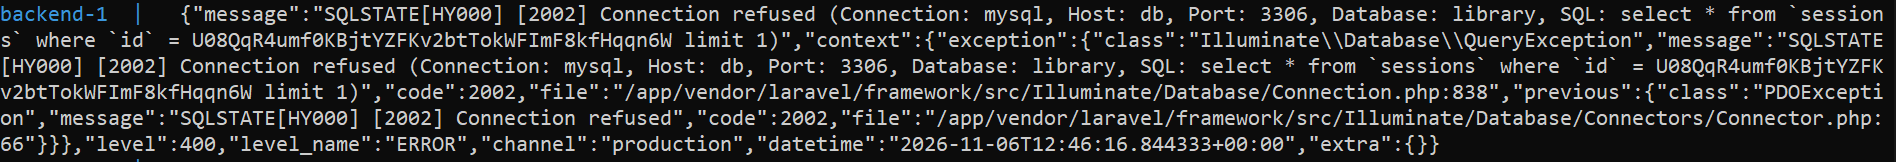
\includegraphics[
    width=\textwidth,
    height=0.30\textheight,
    keepaspectratio,
    trim=950 0 0 0,
    clip
  ]{Screenshot 2026-11-06 194859.png}
  \caption{Log terstruktur ketika koneksi database gagal; detail query dan
  identifier sesi disembunyikan.}
  \label{fig:database-error-log}
\end{figure}

Gambar~\ref{fig:database-error-log} menunjukkan log level \texttt{ERROR} dengan
alasan koneksi ditolak. Konteks tersebut menjelaskan bahwa pemeriksaan database
gagal karena service database tidak dapat dihubungi. Log tidak menampilkan password
atau token.

\section{Bukti Pemulihan}

\screenshot{Screenshot 2026-11-06 194811.png}
{Status service setelah database dinyalakan kembali}
{database-recovered}

Database dinyalakan kembali menggunakan:

\begin{verbatim}
docker compose start db
\end{verbatim}

Gambar~\ref{fig:database-recovered} menunjukkan bahwa database kembali
\texttt{healthy}, kemudian backend dan frontend juga kembali berstatus
\texttt{healthy}. Hal ini membuktikan healthcheck bekerja dua arah: mendeteksi
kegagalan dan mengenali pemulihan.

\section{Ringkasan Hasil}

\begin{table}[H]
\centering
\caption{Ringkasan pemenuhan requirement}
\begin{tabular}{p{0.46\textwidth}p{0.40\textwidth}}
\toprule
\textbf{Requirement} & \textbf{Bukti} \\
\midrule
Log Laravel ke stdout & Gambar~\ref{fig:structured-log} \\
Minimal tiga log terstruktur & Gambar~\ref{fig:structured-log} dan log error \\
Pemeriksaan database dan cache & Gambar~\ref{fig:health-healthy} \\
HTTP 200 saat sehat & Gambar~\ref{fig:health-healthy} \\
HTTP 503 saat database gagal & Implementasi endpoint dan status backend unhealthy \\
Healthcheck Compose dua arah & Gambar~\ref{fig:healthy-services}, \ref{fig:database-stopped}, dan \ref{fig:database-recovered} \\
Rotasi ukuran log & Gambar~\ref{fig:log-rotation} \\
\bottomrule
\end{tabular}
\end{table}

\section{Cara Compile di Overleaf}

Upload dua hal berikut ke project Overleaf:

\begin{enumerate}
  \item file \texttt{P10\_24-540567-SV-24877\_Nawwaf\_Zayyan\_Musyafa.tex};
  \item seluruh folder \texttt{screenshots/} beserta delapan file gambar.
\end{enumerate}

Set \textbf{Main document} ke file \texttt{.tex} ini dan gunakan compiler
\textbf{pdfLaTeX}. Nama file gambar harus dipertahankan sama seperti di folder
\texttt{screenshots/}.

\section{Kesimpulan}

Aplikasi telah memiliki logging terstruktur yang aman, endpoint kesehatan yang
memeriksa dependency nyata, healthcheck Docker Compose dengan parameter lengkap,
serta pembatasan ukuran log. Bukti menunjukkan seluruh service sehat pada kondisi
normal, backend menjadi tidak sehat ketika database dimatikan, error database
tercatat pada log, dan service kembali sehat setelah database dinyalakan.

\end{document}
